\section{Database Schema} \label{section_db}

The DBMS used for the \textbf{SecureBank} application is MySQL. The schema consists of 6 entities or tables. They are 
\begin{enumerate}
\item \textbf{TBL\_CUSTOMER} - This table contains all information about the Customers. These include Profile information, details about login attempts and status of the Customer account.
\item \textbf{TBL\_EMPLOYEE} - This table contains all information about the Employees, such as profile information and status. 
\item \textbf{TBL\_ACCOUNT} - This table consists of details about the Bank Account details of the Customers, such as \textit{Account number} and \textit{Balance}. The referential constraints are implemented in a way that a Customer can hold multiple Accounts in the Bank.
\item \textbf{TBL\_TRANSACTION} - This table holds details of the Transactions performed by all Customers in the Bank. Complete details about the payer and payee(recipient) are recorded here. The constraints are defined so that both parties are account holders of the \textit{SecureBank}.
\item \textbf{TBL\_TRANSACTION\_CODE} - This table contains the Transaction codes (also referred to as \textit{TANs}) corresponding to each Customer. The information about whether the code is already used is also present here.
\item \textbf{TBL\_SCS} - This table consists of the PINs for the Smart Card Simulator, corresponding to each Customer.
\end{enumerate}


Data-types and lengths for all the fields in the tables are carefully chosen, taking into account the purpose and usage in the application. Refer figure \ref{fig:db_schema} for the complete Entity-Relationship diagram of the \textbf{SecureBank} application.\\

In the web application, all queries to the MySQL database are through the PDO interface and in the C part, MySQL prepared statements are used. These mechanisms ensure better performance, safer \& cleaner code along with protection against injection vulnerabilities.

In addition to the usual \textit{Insert}, \textit{Update} and \textit{Update} statements, \textit{\textbf{Transactions}} are also used, mainly in the processing of account transfers. This is due to the fact that a single transfer is associated with multiple actions such as deduction of funds from the sender and depositing funds in the recipient, which involves operations on multiple tables. \textit{Commit} and \textit{Rollback} 
features of Transactions are employed in such scenarios. 

\begin{figure}[ht]
	\centering
	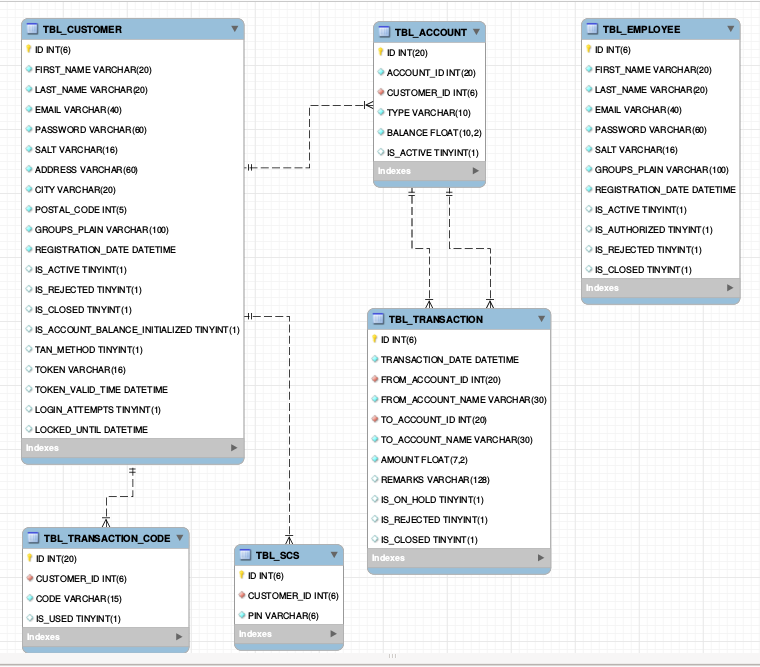
\includegraphics[width=0.9\linewidth]{figures/db_schema.png}
	\caption{Entity-Relationship Diagram of the SecureBank Database}
	\label{fig:db_schema}
\end{figure}

\clearpage